\documentclass[11pt]{article}
\usepackage[utf8]{inputenc}
\usepackage[LGRx,T1]{fontenc}
\usepackage[italian]{babel}
\usepackage{graphicx, wrapfig, multicol}
\usepackage{listings}
\usepackage{color}
\graphicspath{ {./images/} }

\definecolor{dkgreen}{rgb}{0,0.6,0}
\definecolor{gray}{rgb}{0.5,0.5,0.5}
\definecolor{mauve}{rgb}{0.58,0,0.82}

\lstset{frame=tb,
  language=Java,
  aboveskip=3mm,
  belowskip=3mm,
  showstringspaces=false,
  columns=fullflexible,
  basicstyle={\small\ttfamily},
  numbers=left,
  numberstyle=\tiny\color{gray},
  keywordstyle=\color{blue},
  commentstyle=\color{dkgreen},
  stringstyle=\color{mauve},
  breaklines=true,
  breakatwhitespace=true,
  tabsize=1
}

\title{Track My Pantry}
\author{Luca Genova \\ Matricola: 0000882970 \\ Dipartimento di Informatica, Università di Bologna}
\date{\today}

\begin{document}

\maketitle

\null
\null
\null
\null
\section*{Introduzione}
Track my Pantry è un'applicazione sviluppata per il corso di Laboratorio di applicazioni mobili per il C.d.L. di Informatica (a.a. 2020/21).\\
L' obiettivo dell' applicazione è tenere traccia dei prodotti in dispensa attraverso il barcode associato al prodotto, interrogando un Web Service (database condiviso) dove è possibile aggiungere e richiedere i dettagli dei prodotti. In questo report descrivo le principali caratteristiche e le tecniche implementative utilizzate per lo sviluppo.

\newpage
\tableofcontents
\newpage

\section{Dettagli implementativi}
L' applicazione è stata sviluppata per Android in modo ibrido utilizzando Ionic, Capacitor e il framework React. \\
Le chiamate al Web Service sono create mediante la libreria Fetch, per il database è stata utilizzato il plugin SQLite di capacitor e per l'accesso alla fotocamera è stato utilizzato il plugin Camera sempre di capacitor.\\
Il minSdk dell'applicazione è il 23, in quanto il plugin SQLite è supportato dal 23 in poi.\\
Le pagine dell'app sono quattro:
\begin{itemize}
\item Login
\item Registration
\item Home
\item Shopping List
\end{itemize}

L'app si sviluppa fondamentalmente intorno alle due pagine 'Home' e 'Shopping List', le altre due 'Login' e 'Registration' vengono ,ovviamente, utilizzate solo ai fini della login e della registrazione.\\
Sono stati utilizzati solamente componenti Ionic, in modo da rendere l'applicazione il più flessibile possibile.\\
Ho utilizzato la routing di Ionic con una tab bar a tre tab. La prima è la home, la seconda è la shopping list e la terza non è una vera e propria tab ma serve semplicemente per fare il logout.\\
 La pagina di avvio dell'app cambia in base a se l'utente è stato già autenticato o meno (dopo 7 giorni dalla login, l' access token scade), se è autenticato la pagina base sarà /Home altrimenti sarà /Login. \\

\section{Funzionalità}
\subsection{Funzionalità di base}
I requisiti minimi dell'app sono stati tutti sviluppati e sono i seguenti:
\begin{itemize}
\item Aggiornare il database condiviso
\item Effettuare il login e registrarsi per accedere al database remoto
\item Tienere traccia della spesa acquistata
\end{itemize}

\subsection{Funzionalità aggiuntive}
Qui di seguito, invece, troviamo le funzionalità da me aggiunte:
\begin{itemize}
\item Aumento e diminuzione della quantità di un prodotto
\item Barcode scanner
\item Filtrare i prodotti locali per nome
\item Foto per il caricamento di un prodotto
\item Lista della spesa (Shopping list)
\item Immagini dei prodotti
\item Gestione degli utenti diversi
\end{itemize}

\section{Login e Registrazione}
Dalle immagini seguenti si può vedere che sono due pagine molto semplici e molto minimali

\begin{multicols}{2}
\begin{center}
\null \vfill
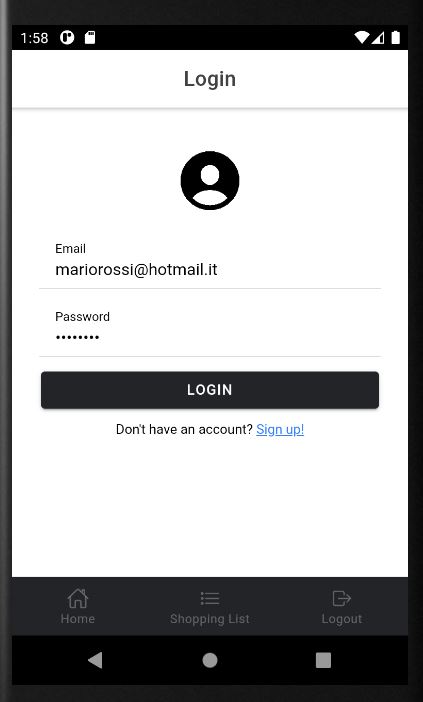
\includegraphics[width=7cm,height=7cm,keepaspectratio]{Login}
\null \vfill
\columnbreak
\null \vfill
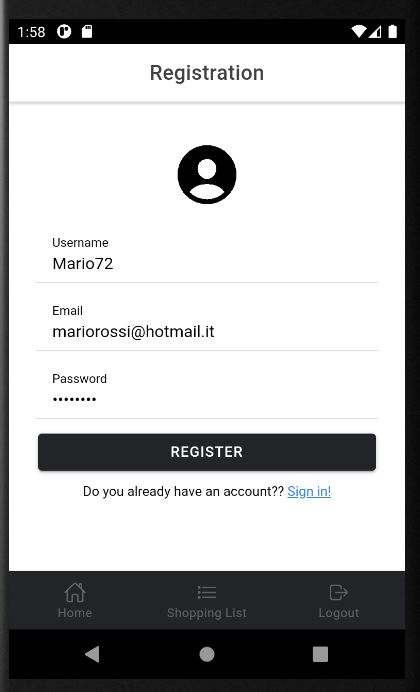
\includegraphics[width=7cm,height=7cm,keepaspectratio]{Registration}
\null \vfill
\end{center}
\end{multicols}


\newpage

\subsection{Login}
Questa pagina contiene due campi:
\begin{enumerate}
\item E-mail
\item Password
\end{enumerate}



Ovviamente finché non verrà eseguito l'accesso, la tab bar rimarrà disabilitata. In caso di successo del login, l'app porterà l'utente nella pagina principale "Home" e abiliterà la tab bar.



\subsubsection{Autenticazione}
Per quanto riguarda l'autenticazione, essa viene gestita memorizzando l'access token al momento del login.\\
Ho utilizzando la libreria "Storage" che mi permette di usufruire delle funzioni get e set per restituire e settare dei valori semplici in memoria. Come si può vedere dall'immagine (righe 14-16), memorizzo l'email, l'access token e la data corrente. La data la utilizzo per controllare la validità dell'access token all'apertura dell'app, dato che dopo 7 giorni scade.

\begin{lstlisting}
export async function login(email: string, password: string) {
    const loginData = {
        email: email,
        password: password
    };
    const requestOptions = {
        method: 'POST',
        headers: { 'Content-Type': 'application/json' },
        body: JSON.stringify(loginData)
    };
    const response = await fetch(baseURL + '/auth/login', requestOptions);
    if(response.ok) {
        const token = await response.clone().json();
        await setValue("accessToken", token);
        await setValue("email", email);
        await setValue("date", new Date());
    }
    return response;
}
\end{lstlisting}

\newpage

\begin{lstlisting}
 export const isAuthed = async () =>{
  const token = await getValue("accessToken");
  const date = new Date(await getValue("date"));
  const today = new Date();
  date.setDate(date.getDate() + 7);
  if(token != null && date.getTime() > today.getTime())
    return true;
  else
    return false;
}
\end{lstlisting}


\subsection{Registrazione}
Questa pagina è molto simile alla precedente. Ha un campo in più per lo username e nel caso la registrazione avvenga con successo l'app porterà l'utente sulla pagina di Login.


\section{Home}
Questa è la sezione principale dell'app, dove c'è una searchbar (filtra i prodotti per nome), un bottone per aggiungere un nuovo prodotto e una IonList che a sua volta contiente tutti i prodotti salvati localmente in un database.\\
La searchbar lavora solo su una copia salvata dei prodotti, quindi non necessita di eseguire ogni volta una query al database locale.

\subsection{Card}
Ogni prodotto viene rappresentato da una card, in cui è presente:

\begin{multicols}{2}
\begin{itemize}
\item Il nome del prodotto
\item La quantità disponibile
\item Due bottoni: uno per aumentare e uno per diminuire la quantità
\columnbreak
\item Un bottone per eliminare definitivamente il prodotto dal database locale
\item Un bottone per altri dettagli del prodotto (finestra con descrizione e barcode)
\end{itemize}
\end{multicols}

\newpage

\begin{figure}
\centering
\begin{minipage}{.5\textwidth}
  \centering
  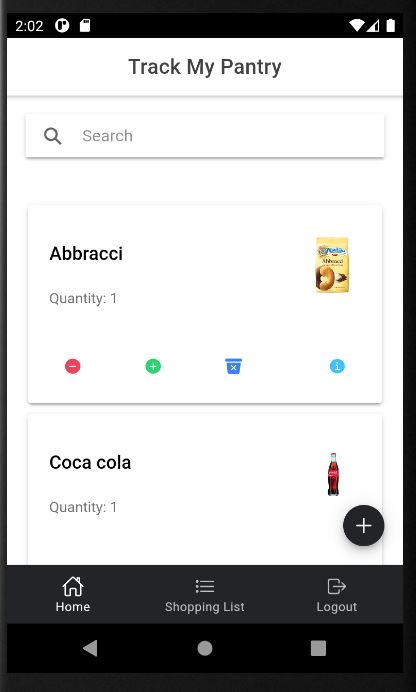
\includegraphics[width=7cm,height=7cm,keepaspectratio]{Home}
\end{minipage}%
\begin{minipage}{.5\textwidth}
  \centering
  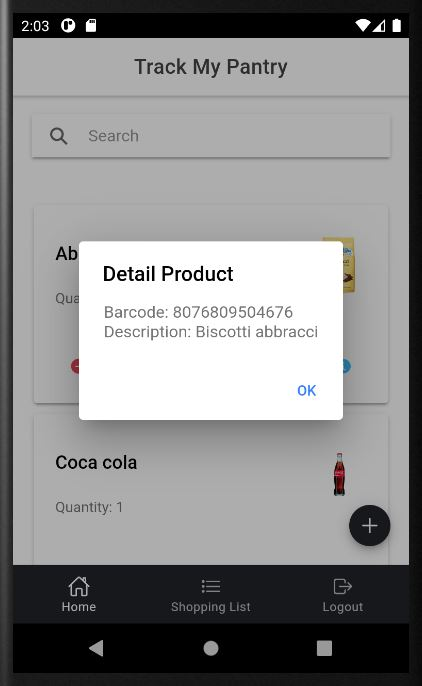
\includegraphics[width=7cm,height=7cm,keepaspectratio]{Home_detail}
\end{minipage}
\end{figure}


La particolarità dell'app sta nel fatto che se la quantità dovesse divenire uguale a 0, la card verrà automaticamente rimossa dalla Home e inserita nella Shopping list. Nel caso venga nuovamente comprato (quindi cercato) quel prodotto, che in quel momento si trova nella Shopping list, verrà reinserito nella Home con quantità = 1 ed eliminato dalla Shopping list.\\
L'idea è quella di dare la possibilità all'utente di eliminare definitivamente un prodotto dalla dispensa, nel caso in cui non se ne faccia più uso, ma anche di mantenerlo se è un prodotto che l'utente compra spesso ma lo ha esaurito.


\subsection{Ricerca del prodotto}
Nel caso si volesse aggiungere un nuovo prodotto alla dispensa, il bottone con l'icona + farà aprire una finestra modale, dove ci sarà la possibilità di cercare nel database condiviso un prodotto tramite barcode (sia stringa che con scannerizzazione del barcode).\\
Il contenuto della finestra è uno stato (utilizzando useState di React) che viene cambiato in base al contesto (scanner, risultati prodotti, creazione di un nuovo prodotto).\\
Il risultato della ricerca saranno sempre delle card simili alle precedenti con tutti i dettagli del prodotto visualizzabili cliccando il bottone di informazione.
A questo punto basta cliccare "ADD" e verrà automaticamente aggiunto il prodotto selezionato con quantità = 1, però solo dopo aver dato un rating da 1 a 5 (partirà una chiamata HTTP per dare il voto al prodotto).
\\
Per la scannerizzazione del barcode ho utilizzato un plugin di Capacitor 'barcode-scanner'.

\begin{figure}
\centering
\begin{minipage}{.5\textwidth}
  \centering
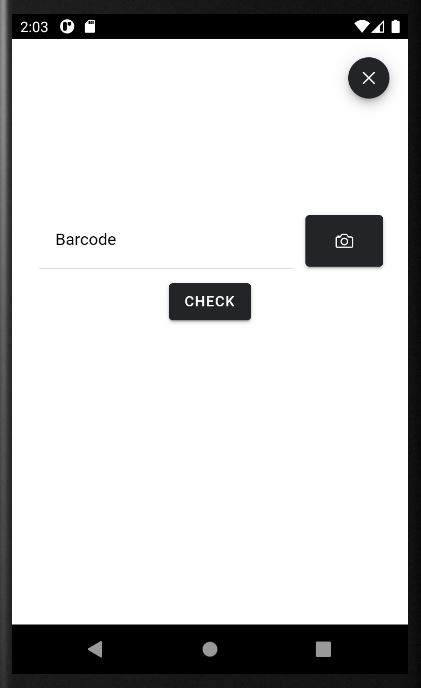
\includegraphics[width=7cm,height=7cm,keepaspectratio]{Barcode}
\end{minipage}%
\begin{minipage}{.5\textwidth}
  \centering
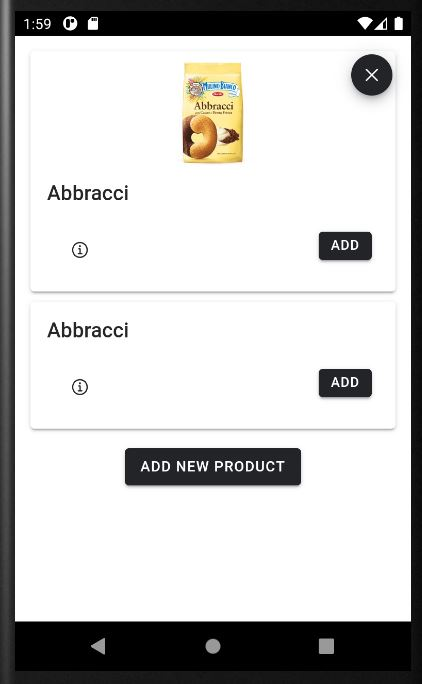
\includegraphics[width=7cm,height=7cm,keepaspectratio]{Product_list}
\end{minipage}
\end{figure}

\subsection{Aggiunta di un nuovo prodotto}

\begin{multicols}{2}
\begin{flushleft}
Se l'utente non è convinto dei prodotti già presenti o il prodotto (barcode) non è  proprio presente nel database remoto, c'è la possibilità di crearne uno.\\
A quel punto si rimarrà sempre sulla stessa finestra modale ma cambierà il contenuto con la possibilità di creare un nuovo prodotto con i seguenti dettagli:
\begin{itemize}
\item Foto scattata in quel momento (opzionale)
\item Nome del prodotto
\item Descrizione del prodotto
\end{itemize}
Dopo aver creato il prodotto, esso verrà automaticamente aggiunto alla dispensa con quantità = 1.
\null \vfill
\end{flushleft}

\columnbreak

\begin{flushright}

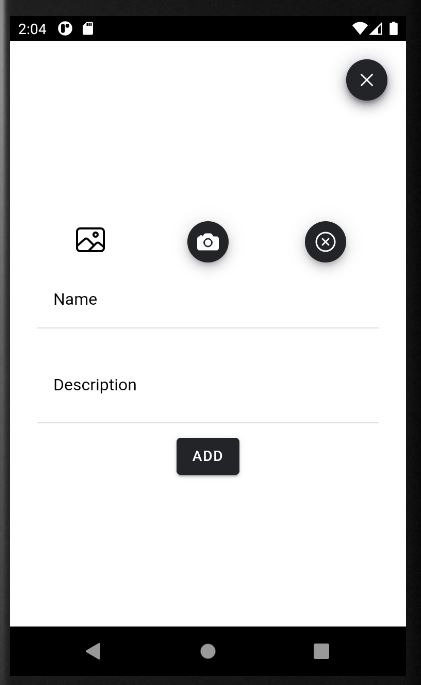
\includegraphics[width=7cm,height=7cm,keepaspectratio]{NewProduct}
\null \vfill
\end{flushright}
\end{multicols}

\newpage


\section{Shopping List}

\begin{multicols}{2}
\begin{flushleft}
In questa sezione dell'app ci sono tutti i prodotti del database locale che hanno quantità = 0.\\
In questo modo riesco a separare per bene i prodotti che ho nella dispensa, con quelli che utilizzo di solito ma sono esauriti.\\
Per aggiornarla di volta in volta utilizzo un evento che viene chiamato ogni qual volta un prodotto raggiunge quantità = 0 o quando viene nuovamente comprato (quindi ricercato nel database condiviso).
\null \vfill
\end{flushleft}

\columnbreak

\begin{flushright}
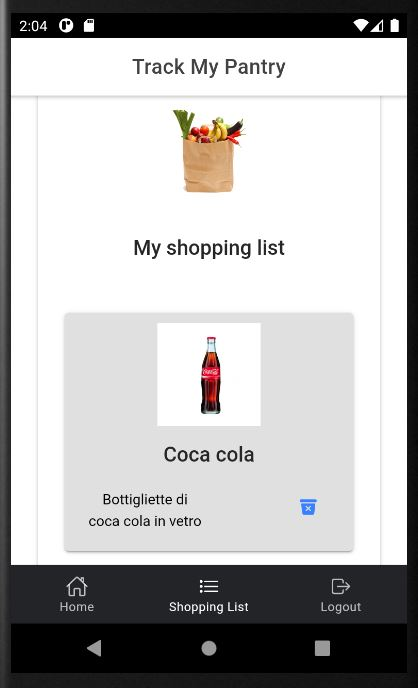
\includegraphics[width=7cm,height=7cm,keepaspectratio]{ShoppingList}
\null \vfill
\end{flushright}
\end{multicols}
 



\section{Gestione utenti diversi}
E’ possibile quindi utilizzare l’applicazione con più utenti diversi ed i prodotti verranno correttamente separati fra questi grazie alla procedura di Login.\\
Questo perché per ogni prodotto memorizzato nel database locale avrà anche il campo e-mail, in modo tale che ogni volta che voglio ottenere i prodotti prenderò solo e soltanto quelli dell'utente corrente, quindi quelli con l'e-mail che combacierà nella query.\\
Infatti ogni volta che l'app esegue una query al database locale, utilizzerà anche l'e-mail dell'utente corrente.

\end{document}}
